% Created by tikzDevice version 0.9 on 2015-12-20 19:43:41
% !TEX encoding = UTF-8 Unicode
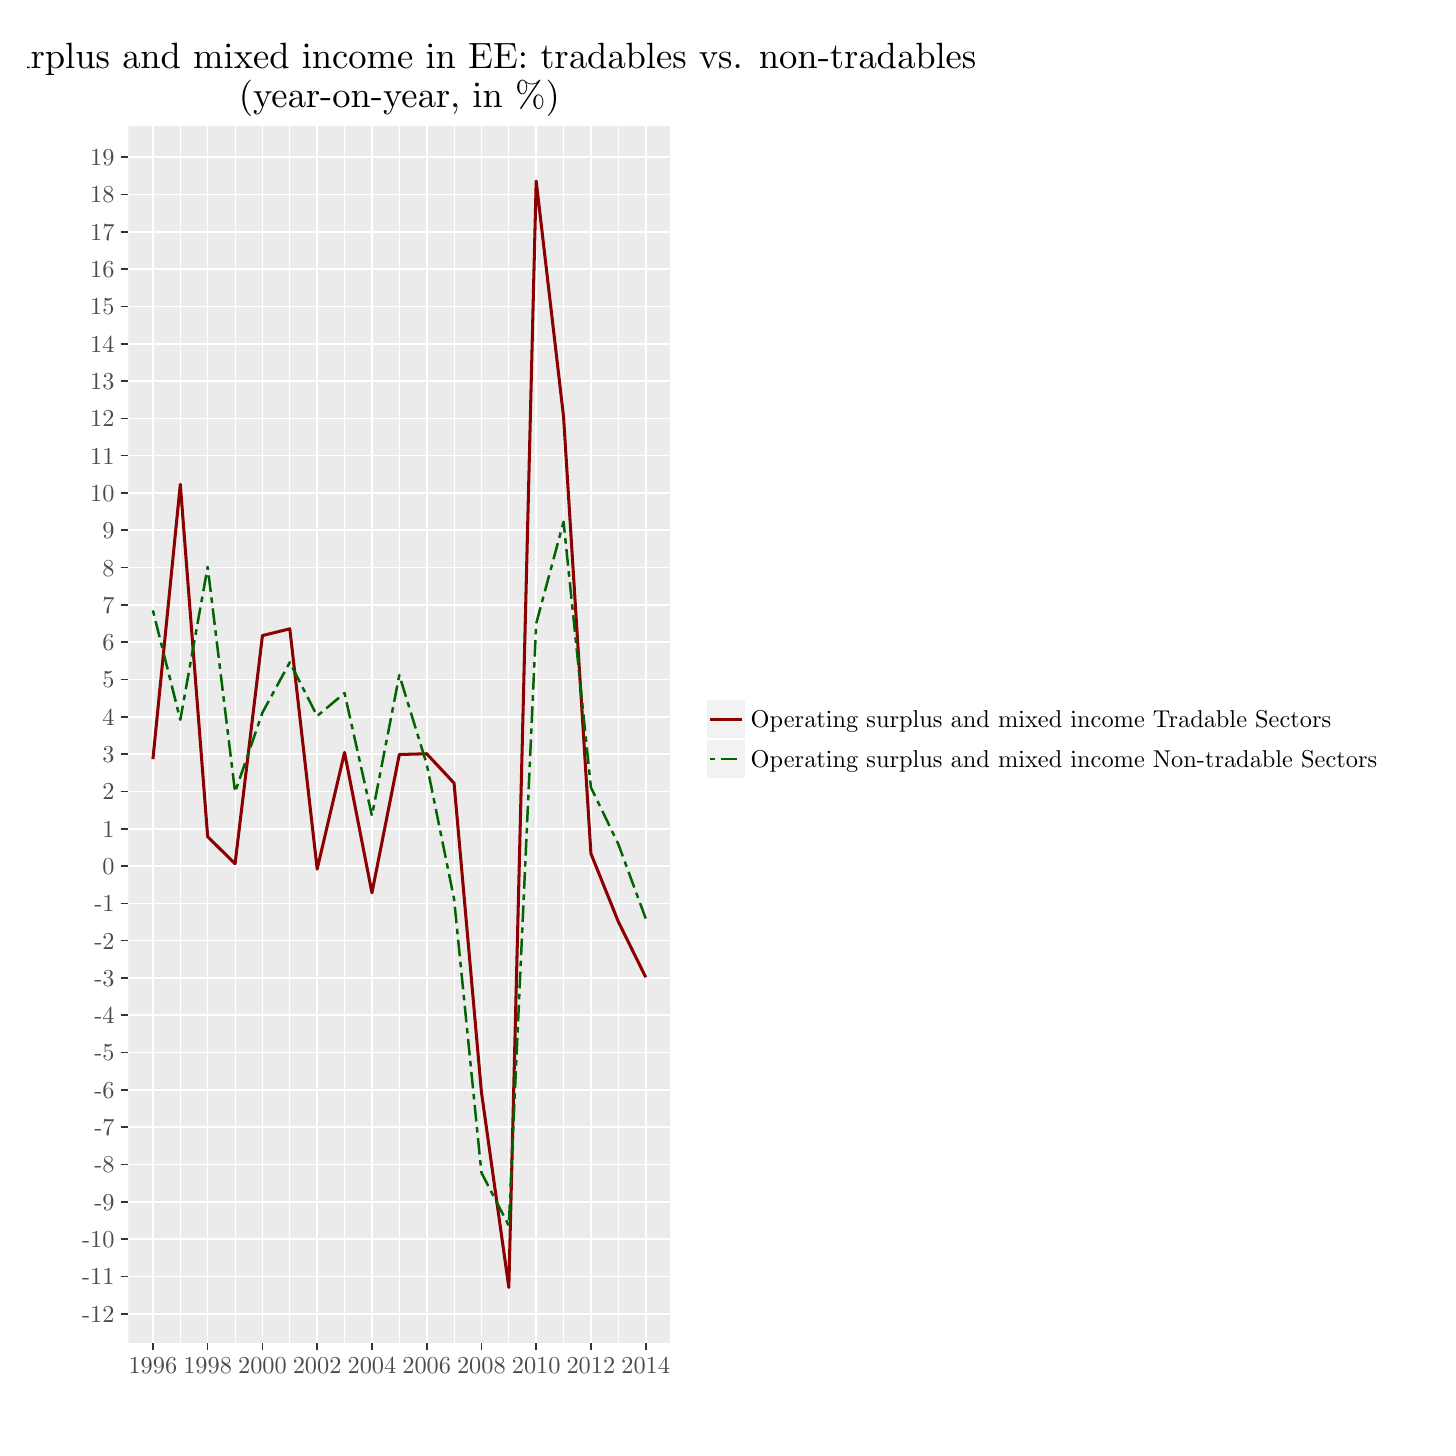
\begin{tikzpicture}[x=1pt,y=1pt]
\definecolor{fillColor}{RGB}{255,255,255}
\path[use as bounding box,fill=fillColor,fill opacity=0.00] (0,0) rectangle (505.89,505.89);
\begin{scope}
\path[clip] (  0.00,  0.00) rectangle (505.89,505.89);
\definecolor{drawColor}{RGB}{255,255,255}
\definecolor{fillColor}{RGB}{255,255,255}

\path[draw=drawColor,line width= 0.6pt,line join=round,line cap=round,fill=fillColor] (  0.00,  0.00) rectangle (505.89,505.89);
\end{scope}
\begin{scope}
\path[clip] ( 36.36, 30.69) rectangle (232.22,470.44);
\definecolor{fillColor}{gray}{0.92}

\path[fill=fillColor] ( 36.36, 30.69) rectangle (232.22,470.44);
\definecolor{drawColor}{RGB}{255,255,255}

\path[draw=drawColor,line width= 0.3pt,line join=round] ( 55.15, 30.69) --
	( 55.15,470.44);

\path[draw=drawColor,line width= 0.3pt,line join=round] ( 74.94, 30.69) --
	( 74.94,470.44);

\path[draw=drawColor,line width= 0.3pt,line join=round] ( 94.72, 30.69) --
	( 94.72,470.44);

\path[draw=drawColor,line width= 0.3pt,line join=round] (114.50, 30.69) --
	(114.50,470.44);

\path[draw=drawColor,line width= 0.3pt,line join=round] (134.29, 30.69) --
	(134.29,470.44);

\path[draw=drawColor,line width= 0.3pt,line join=round] (154.07, 30.69) --
	(154.07,470.44);

\path[draw=drawColor,line width= 0.3pt,line join=round] (173.86, 30.69) --
	(173.86,470.44);

\path[draw=drawColor,line width= 0.3pt,line join=round] (193.64, 30.69) --
	(193.64,470.44);

\path[draw=drawColor,line width= 0.3pt,line join=round] (213.43, 30.69) --
	(213.43,470.44);

\path[draw=drawColor,line width= 0.6pt,line join=round] ( 36.36, 41.17) --
	(232.22, 41.17);

\path[draw=drawColor,line width= 0.6pt,line join=round] ( 36.36, 54.65) --
	(232.22, 54.65);

\path[draw=drawColor,line width= 0.6pt,line join=round] ( 36.36, 68.13) --
	(232.22, 68.13);

\path[draw=drawColor,line width= 0.6pt,line join=round] ( 36.36, 81.62) --
	(232.22, 81.62);

\path[draw=drawColor,line width= 0.6pt,line join=round] ( 36.36, 95.10) --
	(232.22, 95.10);

\path[draw=drawColor,line width= 0.6pt,line join=round] ( 36.36,108.58) --
	(232.22,108.58);

\path[draw=drawColor,line width= 0.6pt,line join=round] ( 36.36,122.06) --
	(232.22,122.06);

\path[draw=drawColor,line width= 0.6pt,line join=round] ( 36.36,135.54) --
	(232.22,135.54);

\path[draw=drawColor,line width= 0.6pt,line join=round] ( 36.36,149.02) --
	(232.22,149.02);

\path[draw=drawColor,line width= 0.6pt,line join=round] ( 36.36,162.50) --
	(232.22,162.50);

\path[draw=drawColor,line width= 0.6pt,line join=round] ( 36.36,175.98) --
	(232.22,175.98);

\path[draw=drawColor,line width= 0.6pt,line join=round] ( 36.36,189.46) --
	(232.22,189.46);

\path[draw=drawColor,line width= 0.6pt,line join=round] ( 36.36,202.94) --
	(232.22,202.94);

\path[draw=drawColor,line width= 0.6pt,line join=round] ( 36.36,216.42) --
	(232.22,216.42);

\path[draw=drawColor,line width= 0.6pt,line join=round] ( 36.36,229.90) --
	(232.22,229.90);

\path[draw=drawColor,line width= 0.6pt,line join=round] ( 36.36,243.38) --
	(232.22,243.38);

\path[draw=drawColor,line width= 0.6pt,line join=round] ( 36.36,256.86) --
	(232.22,256.86);

\path[draw=drawColor,line width= 0.6pt,line join=round] ( 36.36,270.34) --
	(232.22,270.34);

\path[draw=drawColor,line width= 0.6pt,line join=round] ( 36.36,283.82) --
	(232.22,283.82);

\path[draw=drawColor,line width= 0.6pt,line join=round] ( 36.36,297.30) --
	(232.22,297.30);

\path[draw=drawColor,line width= 0.6pt,line join=round] ( 36.36,310.79) --
	(232.22,310.79);

\path[draw=drawColor,line width= 0.6pt,line join=round] ( 36.36,324.27) --
	(232.22,324.27);

\path[draw=drawColor,line width= 0.6pt,line join=round] ( 36.36,337.75) --
	(232.22,337.75);

\path[draw=drawColor,line width= 0.6pt,line join=round] ( 36.36,351.23) --
	(232.22,351.23);

\path[draw=drawColor,line width= 0.6pt,line join=round] ( 36.36,364.71) --
	(232.22,364.71);

\path[draw=drawColor,line width= 0.6pt,line join=round] ( 36.36,378.19) --
	(232.22,378.19);

\path[draw=drawColor,line width= 0.6pt,line join=round] ( 36.36,391.67) --
	(232.22,391.67);

\path[draw=drawColor,line width= 0.6pt,line join=round] ( 36.36,405.15) --
	(232.22,405.15);

\path[draw=drawColor,line width= 0.6pt,line join=round] ( 36.36,418.63) --
	(232.22,418.63);

\path[draw=drawColor,line width= 0.6pt,line join=round] ( 36.36,432.11) --
	(232.22,432.11);

\path[draw=drawColor,line width= 0.6pt,line join=round] ( 36.36,445.59) --
	(232.22,445.59);

\path[draw=drawColor,line width= 0.6pt,line join=round] ( 36.36,459.07) --
	(232.22,459.07);

\path[draw=drawColor,line width= 0.6pt,line join=round] ( 45.26, 30.69) --
	( 45.26,470.44);

\path[draw=drawColor,line width= 0.6pt,line join=round] ( 65.04, 30.69) --
	( 65.04,470.44);

\path[draw=drawColor,line width= 0.6pt,line join=round] ( 84.83, 30.69) --
	( 84.83,470.44);

\path[draw=drawColor,line width= 0.6pt,line join=round] (104.61, 30.69) --
	(104.61,470.44);

\path[draw=drawColor,line width= 0.6pt,line join=round] (124.40, 30.69) --
	(124.40,470.44);

\path[draw=drawColor,line width= 0.6pt,line join=round] (144.18, 30.69) --
	(144.18,470.44);

\path[draw=drawColor,line width= 0.6pt,line join=round] (163.96, 30.69) --
	(163.96,470.44);

\path[draw=drawColor,line width= 0.6pt,line join=round] (183.75, 30.69) --
	(183.75,470.44);

\path[draw=drawColor,line width= 0.6pt,line join=round] (203.53, 30.69) --
	(203.53,470.44);

\path[draw=drawColor,line width= 0.6pt,line join=round] (223.32, 30.69) --
	(223.32,470.44);
\definecolor{drawColor}{RGB}{139,0,0}

\path[draw=drawColor,line width= 1.1pt,line join=round] ( 45.26,241.56) --
	( 55.15,340.87) --
	( 65.04,213.56) --
	( 74.94,203.76) --
	( 84.83,286.22) --
	( 94.72,288.66) --
	(104.61,201.85) --
	(114.50,244.00) --
	(124.40,193.26) --
	(134.29,243.24) --
	(144.18,243.52) --
	(154.07,232.92) --
	(163.96,121.30) --
	(173.86, 50.68) --
	(183.75,450.45) --
	(193.64,365.30) --
	(203.53,207.43) --
	(213.43,182.84) --
	(223.32,162.79);
\definecolor{drawColor}{RGB}{0,100,0}

\path[draw=drawColor,line width= 0.9pt,dash pattern=on 2pt off 2pt on 6pt off 2pt ,line join=round] ( 45.26,295.33) --
	( 55.15,255.78) --
	( 65.04,311.04) --
	( 74.94,229.67) --
	( 84.83,258.39) --
	( 94.72,276.55) --
	(104.61,257.16) --
	(114.50,265.45) --
	(124.40,221.10) --
	(134.29,271.93) --
	(144.18,239.78) --
	(154.07,191.08) --
	(163.96, 92.15) --
	(173.86, 73.00) --
	(183.75,290.56) --
	(193.64,327.36) --
	(203.53,231.36) --
	(213.43,210.85) --
	(223.32,184.01);
\end{scope}
\begin{scope}
\path[clip] (  0.00,  0.00) rectangle (505.89,505.89);
\definecolor{drawColor}{gray}{0.30}

\node[text=drawColor,anchor=base east,inner sep=0pt, outer sep=0pt, scale=  0.88] at ( 31.41, 38.14) {-12};

\node[text=drawColor,anchor=base east,inner sep=0pt, outer sep=0pt, scale=  0.88] at ( 31.41, 51.62) {-11};

\node[text=drawColor,anchor=base east,inner sep=0pt, outer sep=0pt, scale=  0.88] at ( 31.41, 65.10) {-10};

\node[text=drawColor,anchor=base east,inner sep=0pt, outer sep=0pt, scale=  0.88] at ( 31.41, 78.58) {-9};

\node[text=drawColor,anchor=base east,inner sep=0pt, outer sep=0pt, scale=  0.88] at ( 31.41, 92.07) {-8};

\node[text=drawColor,anchor=base east,inner sep=0pt, outer sep=0pt, scale=  0.88] at ( 31.41,105.55) {-7};

\node[text=drawColor,anchor=base east,inner sep=0pt, outer sep=0pt, scale=  0.88] at ( 31.41,119.03) {-6};

\node[text=drawColor,anchor=base east,inner sep=0pt, outer sep=0pt, scale=  0.88] at ( 31.41,132.51) {-5};

\node[text=drawColor,anchor=base east,inner sep=0pt, outer sep=0pt, scale=  0.88] at ( 31.41,145.99) {-4};

\node[text=drawColor,anchor=base east,inner sep=0pt, outer sep=0pt, scale=  0.88] at ( 31.41,159.47) {-3};

\node[text=drawColor,anchor=base east,inner sep=0pt, outer sep=0pt, scale=  0.88] at ( 31.41,172.95) {-2};

\node[text=drawColor,anchor=base east,inner sep=0pt, outer sep=0pt, scale=  0.88] at ( 31.41,186.43) {-1};

\node[text=drawColor,anchor=base east,inner sep=0pt, outer sep=0pt, scale=  0.88] at ( 31.41,199.91) {0};

\node[text=drawColor,anchor=base east,inner sep=0pt, outer sep=0pt, scale=  0.88] at ( 31.41,213.39) {1};

\node[text=drawColor,anchor=base east,inner sep=0pt, outer sep=0pt, scale=  0.88] at ( 31.41,226.87) {2};

\node[text=drawColor,anchor=base east,inner sep=0pt, outer sep=0pt, scale=  0.88] at ( 31.41,240.35) {3};

\node[text=drawColor,anchor=base east,inner sep=0pt, outer sep=0pt, scale=  0.88] at ( 31.41,253.83) {4};

\node[text=drawColor,anchor=base east,inner sep=0pt, outer sep=0pt, scale=  0.88] at ( 31.41,267.31) {5};

\node[text=drawColor,anchor=base east,inner sep=0pt, outer sep=0pt, scale=  0.88] at ( 31.41,280.79) {6};

\node[text=drawColor,anchor=base east,inner sep=0pt, outer sep=0pt, scale=  0.88] at ( 31.41,294.27) {7};

\node[text=drawColor,anchor=base east,inner sep=0pt, outer sep=0pt, scale=  0.88] at ( 31.41,307.75) {8};

\node[text=drawColor,anchor=base east,inner sep=0pt, outer sep=0pt, scale=  0.88] at ( 31.41,321.24) {9};

\node[text=drawColor,anchor=base east,inner sep=0pt, outer sep=0pt, scale=  0.88] at ( 31.41,334.72) {10};

\node[text=drawColor,anchor=base east,inner sep=0pt, outer sep=0pt, scale=  0.88] at ( 31.41,348.20) {11};

\node[text=drawColor,anchor=base east,inner sep=0pt, outer sep=0pt, scale=  0.88] at ( 31.41,361.68) {12};

\node[text=drawColor,anchor=base east,inner sep=0pt, outer sep=0pt, scale=  0.88] at ( 31.41,375.16) {13};

\node[text=drawColor,anchor=base east,inner sep=0pt, outer sep=0pt, scale=  0.88] at ( 31.41,388.64) {14};

\node[text=drawColor,anchor=base east,inner sep=0pt, outer sep=0pt, scale=  0.88] at ( 31.41,402.12) {15};

\node[text=drawColor,anchor=base east,inner sep=0pt, outer sep=0pt, scale=  0.88] at ( 31.41,415.60) {16};

\node[text=drawColor,anchor=base east,inner sep=0pt, outer sep=0pt, scale=  0.88] at ( 31.41,429.08) {17};

\node[text=drawColor,anchor=base east,inner sep=0pt, outer sep=0pt, scale=  0.88] at ( 31.41,442.56) {18};

\node[text=drawColor,anchor=base east,inner sep=0pt, outer sep=0pt, scale=  0.88] at ( 31.41,456.04) {19};
\end{scope}
\begin{scope}
\path[clip] (  0.00,  0.00) rectangle (505.89,505.89);
\definecolor{drawColor}{gray}{0.20}

\path[draw=drawColor,line width= 0.6pt,line join=round] ( 33.61, 41.17) --
	( 36.36, 41.17);

\path[draw=drawColor,line width= 0.6pt,line join=round] ( 33.61, 54.65) --
	( 36.36, 54.65);

\path[draw=drawColor,line width= 0.6pt,line join=round] ( 33.61, 68.13) --
	( 36.36, 68.13);

\path[draw=drawColor,line width= 0.6pt,line join=round] ( 33.61, 81.62) --
	( 36.36, 81.62);

\path[draw=drawColor,line width= 0.6pt,line join=round] ( 33.61, 95.10) --
	( 36.36, 95.10);

\path[draw=drawColor,line width= 0.6pt,line join=round] ( 33.61,108.58) --
	( 36.36,108.58);

\path[draw=drawColor,line width= 0.6pt,line join=round] ( 33.61,122.06) --
	( 36.36,122.06);

\path[draw=drawColor,line width= 0.6pt,line join=round] ( 33.61,135.54) --
	( 36.36,135.54);

\path[draw=drawColor,line width= 0.6pt,line join=round] ( 33.61,149.02) --
	( 36.36,149.02);

\path[draw=drawColor,line width= 0.6pt,line join=round] ( 33.61,162.50) --
	( 36.36,162.50);

\path[draw=drawColor,line width= 0.6pt,line join=round] ( 33.61,175.98) --
	( 36.36,175.98);

\path[draw=drawColor,line width= 0.6pt,line join=round] ( 33.61,189.46) --
	( 36.36,189.46);

\path[draw=drawColor,line width= 0.6pt,line join=round] ( 33.61,202.94) --
	( 36.36,202.94);

\path[draw=drawColor,line width= 0.6pt,line join=round] ( 33.61,216.42) --
	( 36.36,216.42);

\path[draw=drawColor,line width= 0.6pt,line join=round] ( 33.61,229.90) --
	( 36.36,229.90);

\path[draw=drawColor,line width= 0.6pt,line join=round] ( 33.61,243.38) --
	( 36.36,243.38);

\path[draw=drawColor,line width= 0.6pt,line join=round] ( 33.61,256.86) --
	( 36.36,256.86);

\path[draw=drawColor,line width= 0.6pt,line join=round] ( 33.61,270.34) --
	( 36.36,270.34);

\path[draw=drawColor,line width= 0.6pt,line join=round] ( 33.61,283.82) --
	( 36.36,283.82);

\path[draw=drawColor,line width= 0.6pt,line join=round] ( 33.61,297.30) --
	( 36.36,297.30);

\path[draw=drawColor,line width= 0.6pt,line join=round] ( 33.61,310.79) --
	( 36.36,310.79);

\path[draw=drawColor,line width= 0.6pt,line join=round] ( 33.61,324.27) --
	( 36.36,324.27);

\path[draw=drawColor,line width= 0.6pt,line join=round] ( 33.61,337.75) --
	( 36.36,337.75);

\path[draw=drawColor,line width= 0.6pt,line join=round] ( 33.61,351.23) --
	( 36.36,351.23);

\path[draw=drawColor,line width= 0.6pt,line join=round] ( 33.61,364.71) --
	( 36.36,364.71);

\path[draw=drawColor,line width= 0.6pt,line join=round] ( 33.61,378.19) --
	( 36.36,378.19);

\path[draw=drawColor,line width= 0.6pt,line join=round] ( 33.61,391.67) --
	( 36.36,391.67);

\path[draw=drawColor,line width= 0.6pt,line join=round] ( 33.61,405.15) --
	( 36.36,405.15);

\path[draw=drawColor,line width= 0.6pt,line join=round] ( 33.61,418.63) --
	( 36.36,418.63);

\path[draw=drawColor,line width= 0.6pt,line join=round] ( 33.61,432.11) --
	( 36.36,432.11);

\path[draw=drawColor,line width= 0.6pt,line join=round] ( 33.61,445.59) --
	( 36.36,445.59);

\path[draw=drawColor,line width= 0.6pt,line join=round] ( 33.61,459.07) --
	( 36.36,459.07);
\end{scope}
\begin{scope}
\path[clip] (  0.00,  0.00) rectangle (505.89,505.89);
\definecolor{drawColor}{gray}{0.20}

\path[draw=drawColor,line width= 0.6pt,line join=round] ( 45.26, 27.94) --
	( 45.26, 30.69);

\path[draw=drawColor,line width= 0.6pt,line join=round] ( 65.04, 27.94) --
	( 65.04, 30.69);

\path[draw=drawColor,line width= 0.6pt,line join=round] ( 84.83, 27.94) --
	( 84.83, 30.69);

\path[draw=drawColor,line width= 0.6pt,line join=round] (104.61, 27.94) --
	(104.61, 30.69);

\path[draw=drawColor,line width= 0.6pt,line join=round] (124.40, 27.94) --
	(124.40, 30.69);

\path[draw=drawColor,line width= 0.6pt,line join=round] (144.18, 27.94) --
	(144.18, 30.69);

\path[draw=drawColor,line width= 0.6pt,line join=round] (163.96, 27.94) --
	(163.96, 30.69);

\path[draw=drawColor,line width= 0.6pt,line join=round] (183.75, 27.94) --
	(183.75, 30.69);

\path[draw=drawColor,line width= 0.6pt,line join=round] (203.53, 27.94) --
	(203.53, 30.69);

\path[draw=drawColor,line width= 0.6pt,line join=round] (223.32, 27.94) --
	(223.32, 30.69);
\end{scope}
\begin{scope}
\path[clip] (  0.00,  0.00) rectangle (505.89,505.89);
\definecolor{drawColor}{gray}{0.30}

\node[text=drawColor,anchor=base,inner sep=0pt, outer sep=0pt, scale=  0.88] at ( 45.26, 19.68) {1996};

\node[text=drawColor,anchor=base,inner sep=0pt, outer sep=0pt, scale=  0.88] at ( 65.04, 19.68) {1998};

\node[text=drawColor,anchor=base,inner sep=0pt, outer sep=0pt, scale=  0.88] at ( 84.83, 19.68) {2000};

\node[text=drawColor,anchor=base,inner sep=0pt, outer sep=0pt, scale=  0.88] at (104.61, 19.68) {2002};

\node[text=drawColor,anchor=base,inner sep=0pt, outer sep=0pt, scale=  0.88] at (124.40, 19.68) {2004};

\node[text=drawColor,anchor=base,inner sep=0pt, outer sep=0pt, scale=  0.88] at (144.18, 19.68) {2006};

\node[text=drawColor,anchor=base,inner sep=0pt, outer sep=0pt, scale=  0.88] at (163.96, 19.68) {2008};

\node[text=drawColor,anchor=base,inner sep=0pt, outer sep=0pt, scale=  0.88] at (183.75, 19.68) {2010};

\node[text=drawColor,anchor=base,inner sep=0pt, outer sep=0pt, scale=  0.88] at (203.53, 19.68) {2012};

\node[text=drawColor,anchor=base,inner sep=0pt, outer sep=0pt, scale=  0.88] at (223.32, 19.68) {2014};
\end{scope}
\begin{scope}
\path[clip] (  0.00,  0.00) rectangle (505.89,505.89);
\definecolor{fillColor}{RGB}{255,255,255}

\path[fill=fillColor] (240.76,230.04) rectangle (491.85,271.09);
\end{scope}
\begin{scope}
\path[clip] (  0.00,  0.00) rectangle (505.89,505.89);
\definecolor{drawColor}{RGB}{255,255,255}
\definecolor{fillColor}{gray}{0.95}

\path[draw=drawColor,line width= 0.6pt,line join=round,line cap=round,fill=fillColor] (245.02,248.76) rectangle (259.48,263.21);
\end{scope}
\begin{scope}
\path[clip] (  0.00,  0.00) rectangle (505.89,505.89);
\definecolor{drawColor}{RGB}{139,0,0}

\path[draw=drawColor,line width= 1.1pt,line join=round] (246.47,255.99) -- (258.03,255.99);
\end{scope}
\begin{scope}
\path[clip] (  0.00,  0.00) rectangle (505.89,505.89);
\definecolor{drawColor}{RGB}{255,255,255}
\definecolor{fillColor}{gray}{0.95}

\path[draw=drawColor,line width= 0.6pt,line join=round,line cap=round,fill=fillColor] (245.02,234.30) rectangle (259.48,248.76);
\end{scope}
\begin{scope}
\path[clip] (  0.00,  0.00) rectangle (505.89,505.89);
\definecolor{drawColor}{RGB}{0,100,0}

\path[draw=drawColor,line width= 0.9pt,dash pattern=on 2pt off 2pt on 6pt off 2pt ,line join=round] (246.47,241.53) -- (258.03,241.53);
\end{scope}
\begin{scope}
\path[clip] (  0.00,  0.00) rectangle (505.89,505.89);
\definecolor{drawColor}{RGB}{0,0,0}

\node[text=drawColor,anchor=base west,inner sep=0pt, outer sep=0pt, scale=  0.88] at (261.28,252.95) {Operating surplus and mixed income Tradable Sectors};
\end{scope}
\begin{scope}
\path[clip] (  0.00,  0.00) rectangle (505.89,505.89);
\definecolor{drawColor}{RGB}{0,0,0}

\node[text=drawColor,anchor=base west,inner sep=0pt, outer sep=0pt, scale=  0.88] at (261.28,238.50) {Operating surplus and mixed income Non-tradable Sectors };
\end{scope}
\begin{scope}
\path[clip] (  0.00,  0.00) rectangle (505.89,505.89);
\definecolor{drawColor}{RGB}{0,0,0}

\node[text=drawColor,anchor=base,inner sep=0pt, outer sep=0pt, scale=  1.32] at (134.29,491.30) {Operating surplus and mixed income in EE: tradables vs. non-tradables };

\node[text=drawColor,anchor=base,inner sep=0pt, outer sep=0pt, scale=  1.32] at (134.29,477.04) { (year-on-year, in {\%})};
\end{scope}
\end{tikzpicture}
